\documentclass[a4paper, 11pt]{article}

\usepackage[greek, francais]{babel}
\usepackage[T1]{fontenc}
\usepackage[utf8]{inputenc}
\usepackage[top=4cm, bottom=4cm, left=3cm, right=3cm]{geometry}
\usepackage{qsymbols}
\usepackage{graphicx}
\usepackage{amsmath}
\usepackage{hyperref}
\usepackage{fancyhdr}


\begin{document}

%la premiere page du document

\begin{titlepage}

\includegraphics[width=5cm]{images/logo_mines.jpg}
\vspace{6cm}
\begin{center}
\hrulefill\\
{\LARGE \textbf{RAPPORT DE PROJET 3ème ANNÉE\\ - La statistique des petits nombres -\\}}
\hrulefill\\

\vspace{1cm}

{\Large Détection de comportement atypique à partir d'historiques de navigation Internet d'un groupe d'individus}
\vspace{2cm}

\begin{minipage}{5cm}
\begin{center}
\textbf{Auteur:}\\
LAUWERIERE Fabrice
\end{center}
\end{minipage}
\hspace{1cm}
\begin{minipage}{5cm}
\begin{center}
\textbf{Tutrice de projet :}\\
BENMOUFFEK Dominique
\end{center}
\end{minipage}
\end{center}
\end{titlepage} 

%La table des matieres
\tableofcontents


%====================
%les entete et pieds de page
%====================


\pagestyle{fancy}
\fancyhead[L]{\leftmark}
\fancyhead[C]{}
\fancyhead[R]{}
\fancyfoot[L]{\textbf{Rapport de stage 2A - École des Mines de Nancy}}
\fancyfoot[C]{}
\fancyfoot[R]{\thepage}



%INTRODUCTION
\newpage

\section{Introduction : Étude bibliographique et définition du sujet de recherche}

\subsection{Travaux sur l'utilisation des données de navigation}
Une des particularités du début de ce projet a été le besoin de choisir et de définir l'objet de recherche du projet. En effet les seules directions données étaient qu'il devait se baser sur l'analyse de traces récupérer sur Internet ou bien sur des algorithme de recommandation pour de faible population.

La première phase de ce projet a donc été une étude bibliographique afin de mieux cerner et de mieux comprendre les enjeux de ces domaines. L'élément déclencheur qui m'a fait choisir de travailler sur la détection de comportement atypique à partir des données de navigation internet d'un groupe d'individus a été la lecture d'une publication de Eugene A\textsc{gichtein} : \href{http://www.cse.lehigh.edu/academics/graduate-programs/graduate-computer-engineering/2-uncategorised/235-agichtein}{Mining Online User Behavior: from Improving Search to Detecting Cognitive Impairment}. Ce papier décrit l'idée d'utiliser et d'analyser le comportement d'individus sur internet pour tenter de repérer chez eux des signes de maladies cognitives comme la maladie d'Alzheimer.

\subsection{La détection de comportement atypique : parallèle avec la génétique}

Ayant déjà utilisé des algorithmes de génétique pour d'autres projet, j'ai pensé essayer d'adapter et d'identifier mon problème à un problème de génétique. Les avantages apportés par l'utilisation d'un algorithme de génétique sont tout d'abord la documentation par rapport à ces algorithmes puisqu'ils sont pour la plupart utilisés depuis assez longtemps. 

La détection de mutations et de singularités est aussi un des principaux problèmes de la génétique et j'ai pensé qu'il serait possible de transposer le problème qui m'intéresse à un problème de génétique de ce type. Nous verrons un peu plus tard comment cette transposition a été faite.

\section{Génération des données de travail}

\subsection{Impossibilité de récupérer de vraies données}
Pour pouvoir essayer de détecter un comportement atypique d'un individu au milieu d'une population qui elle aurait un comportement qu'on appellera normal, il faut avoir cette référence de la navigation internet classique d'un individu. Pour récupérer des historique de navigation, on peut penser soit les récupérer en les demandant à de vraies personnes mais l'inconvénient principal de cette technique est que l'on obtiendrait pas un nombre suffisant d'historiques pour pouvoir travailler dessus. 

La seconde possibilité rapidement abandonnée était de récupérer ces historiques à l'insu des personnes concernées grâce à du spam. Cette solution sortant du cadre légal et étant assez complexe à tout de suite été écartée.\\

La solution restante est de générer des individus et leurs historiques. Le problème principal devient alors la création d'historique de navigation plausible et le plus proche possible de la navigation qu'aurait un vrai être humain.

\subsection{Récupération en ligne de données par un robot}

Les matières premières pour créer des historiques les plus réalistes possibles sont les statistiques et les informations sur les sites internet les plus visités. Toutes ces informations ont été récupérées sur le site \href{http://www.alexa.com/siteinfo}{Alexa.com} qui fournit des informations et des statistiques sur le trafic des sites internet. Ce site fournit également des classements des sites par rapport à leur nombre de visiteurs.

On a donc créer un robot qui récupère les informations voulues envoyant une requête HTTP et en parsant le code html de la page pour en extraire les information voulues. Ces informations sont ensuite stockées au fur et à mesure dans un fichier XML. Cette récupération se fait en plusieurs étapes comme décrit ci-après : \\
\begin{itemize}
\item[•] On récupère en premier le classement des 500 premiers sites les plus visités en France. (Remarque : On a utilisé la France mais il suffit de changer l'adresse de requête pour pouvoir travailler avec des données sur un autre pays)
\item[•] Une fois que l'on a récupéré les 500 sites les plus visités et qu'ils sont stockés dans un XML par rang, on parcours ce fichier XML et pour chacun des sites on effectue une requête HTTP vers la page des informations détaillés sur ce site. On récupère alors dans le code html de la page les 10 parents dans la navigation qui sont les plus probables ainsi que leur pourcentage. Un parent dans la navigation est un site qu'un internaute a visité juste avant de visiter le site en question. Le pourcentage cité est le pourcentage de gens arrivant sur ce site depuis le parent en question. On stocke chacun de ces parents dans le fichier XML
\item[•] Sur la même page d'informations détaillées sur chacun des 500 sites, on récupère aussi les principales catégories auxquelles le site appartient. Ces principales catégories sont également stockées dans le fichier XML à la suite des parents de navigation.
\end{itemize}~\\

Avec une connexion internet d'environ 10 mega, le robot à besoin d'une douzaine de minutes pour récupérer toutes les informations voulues et les stocker. Voici un aperçu des informations recueillies dans le XML pour un site internet.

\begin{figure}[h!]
\center
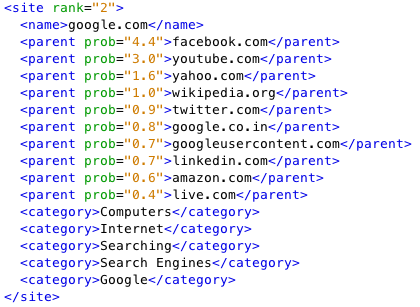
\includegraphics[width=9cm]{images/infoSiteXML.png}
\caption{Information sur un site internet stocké dans un fichier XML par le robot}
\end{figure}

Ce robot n'a besoin d'être lancé qu'une seule fois mais on peut le lancer plusieurs fois pour des informations sur des pays différents si l'on souhaite faire des comparaisons.


\subsection{Création d'historique pour un groupe d'individus}
\subsubsection{Les racines pour des branches de navigation}
Pour la création d'historiques les plus "humains" possible, on considère que les individus fonctionnent par session de navigation que l'on appellera des branches. Une branche correspond au fait que l'individu va aller sur un premier site puis naviguer depuis ce site racine vers d'autres site qui sont chacun assez proche de leur prédécesseur. Le programme demande donc en tout premier lieu le nombre d'individus pour lesquels on souhaite créer un historique puis il sera demandé à l'utilisateur un nombre minimum et un maximum de racines pour les individus du groupe. Pour chaque individu du groupe le programme tirera ensuite aléatoirement un nombre entre ces deux bornes qui déterminera le nombre de branche de navigation dans l'historique.
Chaque racine est choisie aléatoirement parmi les 50 premiers sites les plus visités.

\subsubsection{La profondeur des branches}

Le programme demandera également à l'utilisateur de lui donner une profondeur minimum et maximum pour les branches de navigation. Pour chaque individu et chaque branche de cet individu, une profondeur sera tirer aléatoirement entre les bornes rentrées. Cette profondeur correspond au nombre de fois qu'un utilisateur va passer d'un site à un successeur. Il faut faire remarquer deux choses: 
\begin{itemize}
\item Tout d'abord le fait que l'on créé ces branches de navigation à l'envers, on part du dernier site visité et on remonte vers un des 10 premiers parents de ce site car les seules informations que nous avons sont les parents des sites. Le parent vers lequel on remonte parmi les 10 est choisi aléatoirement mais ce choix est pondéré par les probabilités de chacun de ces parents.
\item Ensuite il en résulte que si l'on choisi un parent qui ne figure pas dans la liste des 500 premiers sites les plus visités sur lesquels on possède des informations, on ne peux pas choisir un nouveau parent malgré le fait que l'on n'ait pas encore atteint la profondeur atteinte. On imagine alors un système de repêchage décrit ci-après.
\end{itemize}

\subsubsection{Le repêchage en cas de manque d'informations}

Si l'on est dans le cas décrit ci-avant où le dernier parent choisi dans la branche de navigation ne fait pas partie de la liste de sites pour lesquels on possède des informations, on défini un système de repêchage qui consiste à donner à la branche en question une chance de repartir sur un des 20 premiers sites les plus visité. Cette chance est proportionnelle à l'avancement dans la profondeur de la branche. Plus on est arrivé loin dans la branche et moins on a de chance d'être repêché.

Si la branche en question ne passe pas le repêchage, elle est arrêtée avant d'atteindre la profondeur qui lui avait été assignée.

\subsection{Classement des données par catégories}

\subsubsection{Établissement et indexation d'une liste des catégories}

L'algorithme que l'on va utiliser et qui sera détaillé un peu plus loin dans ce rapport a besoin en entrée du nombre de site de chaque catégorie pour tous les individus. Une fois que l'on a les données de navigation pour tous les individus, on créé alors en parcourant le fichier XML des 500 premiers site une liste de toutes les catégories de site possibles et on compte pour chaque utilisateur le nombre de sites de chaque catégories qu'il a visité.

\subsubsection{Pertinence du classement et des catégories retenues}

On peut s'interroger sur la pertinence d'un tel classement par catégories. En effet les catégories récupérées sur le site \href{http://www.alexa.com/siteinfo}{Alexa.com} sont quelquefois peu commune en particulier lorsqu'il s'agit de site internet étrangers. Certaines catégories ne sont même pas écrites avec des caractères de l'alphabet latin. Cependant ce qui nous intéressera plus tard dans l'algorithme, se sera seulement si pour une ou plusieurs catégories, un ou plusieurs individu ont des comportement qui diffèrent beaucoup des autres. Étant donné cela, des catégories sans noms et simplement numérotées auraient suffis.

La deuxième chose sur laquelle on peut avoir des doutes quand au classement par catégories, c'est la fait que tous les sites qui sont dans l'historique mais qui ne font pas partie des 500 premiers sur lesquels on a des infos ne seront pas classés. On peut relativiser cela par le fait que l'on ne rencontre ce cas que très rarement.

\subsection{L'insertion des cas atypiques}

Une fois que le classement des sites visités par catégories est fait pour chaque individu, il est demandé à l'utilisateur de choisir un nombre d'individus auxquels on souhaite conférer un comportement atypique. Il a été choisi de ne pas laisser la possibilité à l'utilisateur de modifier plus de 50\% des individus pour deux raisons. Tout d'abord la vraisemblance mais aussi le fait que cela permet de réduire grandement le nombre de cas à traiter et donc le temps de calcul de l'algorithme.

On a choisi de créer un comportement atypique en ajoutant à un individu sur une, deux ou trois catégories un nombre de visite supplémentaire allant de 100 à 200 (tiré aléatoirement). On peut bien sûr créer des comportements atypique de manière différente mais ce cas là m'a paru le plus adapté pour un premier essai.


\section{Utilisation d'un algorithme de génétique}
\subsection{Origine : évolution génétique et analyse de fichiers d'audits de sécurité}

Comme cela a été mentionné plus haut, l'idée d'utiliser un algorithme de génétique pour détecter les comportement atypiques parait pertinente pour deux raison principale. Tout d'abord le fait qu'en génétique le problème de détection de mutation expliquant l'évolution d'une population peut être transposé à notre problème. La deuxième raison est que les algorithmes de génétique sont depuis maintenant assez longtemps connus et ont été optimisés.

Pour ce projet, une publication de Ludovic MÉ, \href{http://www.rennes.supelec.fr/ren/perso/lme/PUBLI/raid98.pdf}{\emph{GasSATA, a Genetic Algorithm as an Alternative Tool for Security Audit Trails Analysis}} a beaucoup aidé à comprendre l'algorithme et surtout à le transposer au problème traité puisque dans ce papier, l'algorithme génétique qui nous intéresse  a été transposer pour la résolution du problème de l'audit e fichiers de sécurité sur un système informatique. En résumé, on cherche dans ce problème la combinaison d'attaque la plus probable pour expliquer les fichiers d'audits.


\subsection{Fonctionnement de l'algorithme}

\subsubsection{Quelques notations}
Pour l'explication de l'algorithme, on utilisera un schéma tiré du papier de Ludovic MÉ cité précédemment ainsi que les mêmes notations pour des raisons de commodité.\\

\textbf{$N_a$} représente dans le papier le nombre d'attaques possible que peut subir le système. Dans notre cas il représentera le nombre de personnes dans le groupe que l'on évalue. On cherchera alors la meilleure combinaison de personnes atypique pour expliquer les observations.\\

\textbf{$N_e$} représente dans le papier les différents types d'événements qui peuvent survenir dans chaque attaque. Pour nous ce nombre représentera donc le nombre de différentes catégories de sites possiblement visitables par un individu.\\

\textbf{AE} sera la matrice des occurrences. C'est la matrice de taille $N_e$ x $N_a$ qui contient pour chaque individu le nombre de sites de chaque catégories qu'il a visité.\\

\textbf{R} est une matrice de taille $N_a$ qui contient les risques pour le système regardant chaque attaque. Transposé à notre problème, cette matrice représenterait le risque encouru si tel ou tel individu est atypique. Vu qu'il n'y en a pas, tous les individu seront considérés comme ayant un même risque de 1.\\

\textbf{H} est une matrice binaire de taille $N_a$ dont les valeurs sont 1 si l'individu est atypique et 0 sinon. C'est cette matrice H la meilleure possible que l'on cherchera.\\

\textbf{O} est la matrice des observations. Dans notre cas cette matrice correspondra a une matrice de taille $N_e$ qui contiendra le nombre de site visité par catégorie pour tout individu confondu s'il n'y avait eu aucun cas atypique.


\subsubsection{L'algorithme}

Le but de l'algorithme est de maximisé le produit entre les matrices R et H tout en respectant les conditions que pour chaque catégorie, le produit AE x H doit être inférieur ou égal  à O. On voit que cette condition sera respectée mais peut ne pas l'être si la matrice H contient un 1 pour un ou plusieurs individu atypique. C'est ce que l'on utilisera pour les détecter. On peut donc résumé avec le schéma suivant tiré du papier de Ludovic MÉ, \href{http://www.rennes.supelec.fr/ren/perso/lme/PUBLI/raid98.pdf}{\emph{GasSATA, a Genetic Algorithm as an Alternative Tool for Security Audit Trails Analysis}}.

\begin{figure}[h!]
\center
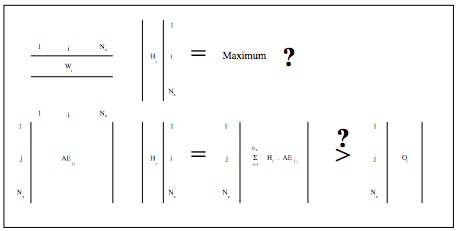
\includegraphics[width=9cm]{images/algoSchema.png}
\caption{Schéma résumant l'algorithme GASSATA}
\end{figure}

\subsubsection{La fonction de sélection}

Afin de rechercher la meilleure combinaison possible, on va définir une fonction dite de sélection pour chaque combinaison possible du vecteur H. Le but sera alors de trouver le maximum de cette fonction. Vu que ce que l'on cherche à maximiser est le produit R.H, le calcul de la fonction contiendra ce produit. 

On va ensuite définir des pénalités qui vont faire diminuer la valeur prise par cette fonction dans les cas où certaines des catégories ne respectent pas l'inégalité. On aura une fonction de sélection de la forme suivante : \\

\begin{figure}[h!]
\center
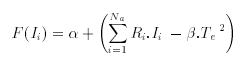
\includegraphics[width=6cm]{images/fonctionSelection.png}
\caption{Forme de la fonction de sélection}
\end{figure}

Ici la matrice I représente une des combinaisons possibles de la matrice H recherchée. $T_e$ représente le nombre de catégories qui ne respectent pas l'inégalité et qui entraîneront donc une pénalité. Cette pénalité est représentée par le produit $\beta T_e^2$. Le coefficient $\alpha$ sert à faire en sorte qu'à partir d'un certain nombre de catégories pénalisées, la fonction renvoi une valeur négative et la solution I sera alors écartée. 

\subsubsection{Utilisation de nombres binaires}

Comme cela a déjà été dit précédemment, on ne testera pas tous les cas possible mais seulement les cas avec au plus 50\% d'individus atypique parmi le groupe.

Toutes les combinaisons possible pour le vecteur H sont les représentation binaire des nombres allant de 0 à $2^{N_a}$. Parmi toutes ces possibilités, on ne teste donc que celles qui ont au plus $\frac{N_a}{2}$ 1 et le reste de 0.

\subsubsection{La récupération du(des) meilleur(s) résultat}

On récupère donc en sortie de l'algorithme toutes les combinaisons pour lesquelles la fonction de sélection est positive. Cela correspond à toutes les solutions où au moins un individu atypique a été détecté. 

Dans la formule de la fonction de sélection, la puissance de $T_e$ sert justement à séparer les groupes de résultats en fonction du nombre d'individus atypiques détectés. Plus on détecte d'individus atypiques et plus la valeur prise par la fonction sera grande mais les valeurs prisent par la fonction pour des cas où l'on détecte le même nombre d'atypiques seront proche.

On récupère donc le paquet de résultat le plus grand qui correspond aux combinaison ayant détecté le plus d'individus atypiques. Ensuite parmi ces différentes possibilités, il faut choisir la meilleure, c'est à dire celle qui ne considère pas en plus comme atypique des individus qui ne le sont pas. Ce sera donc la combinaison qui possède le moins de 1 possible parmi le groupe déjà présélectionné. Cela se traduit par la valeur la plus basse de la fonction de sélection dans ce groupe.

\subsection{Temps de calcul et complexité}

La complexité de cet algorithme est exponentielle. En effet le temps de calcul de cet algorithme dépend principalement du nombre d'individus dans le groupe que l'on souhaite tester. En effet, à chaque fois que l'on rajoute 1 individu supplémentaire, on multiplie le temps de calcul par 2 environ.

Ainsi compte tenu du fait que l'on à ici 410 catégories différentes, avec un processeur de 2,9 GHz et un mémoire de 8 Go, on obtient les temps de calcul suivants :

\begin{figure}[h!]
\center
\begin{tabular}{|c|c|}
\hline
$N_a$ & Temps\\
\hline
3 & 10s\\
\hline
5 & 55s\\
\hline
7 & 3m40s\\
\hline
10 & 35m\\
\hline
12 & 2h40m\\
\hline
\end{tabular}
\caption{Tableau des temps de calcul en fonction du nombre d'individus}
\end{figure}

On peut donc à partir de là faire des estimations de ce temps de calcul si l'on considère des plus grands groupes d'individus.

\begin{figure}[h!]
\center
\begin{tabular}{|c|c|}
\hline
$N_a$ & Temps estimé\\
\hline
15 & 24h\\
\hline
20 & 32j\\
\hline
30 & 90ans\\
\hline
\end{tabular}
\caption{Tableau des temps de calcul en fonction du nombre d'individus}
\end{figure}

\subsection{Validité des résultats}

La validité des résultats dépend principalement de la matrice de référence O que l'on va considérer. Si l'on construit cette matrice à partir des informations de navigation produites avant l'insertion d'individus à comportement atypique, avec les coefficients $\alpha$ et $\beta$ ainsi que la puissance choisis correctement pour éliminer toutes les combinaisons qui n'ont que des pénalités sur toutes les catégories, le résultat obtenu sera à chaque fois le bon. 

Par contre si on considère le cas plus réaliste d'une matrice de référence calculée en faisant la moyenne de plusieurs créations d'historiques avec des paramètres similaires à ceux de l'historique que l'on souhaite étudier, sauf cas particulier faiblement probable, on obtiendra les combinaisons regroupant tous les cas atypiques mais il sera difficile de différencier la solution optimale de celles où l'on a des individus normaux considérés comme atypiques.

\subsection{Piste explorée sans succès}

Avant l'utilisation de l'algorithme ci-avant, il a été tenté de réaliser la détection à l'aide de fonctions de notations qui permettraient de noté le risque que représente chaque catégorie pour le comportement recherché en fonction du nombre de visite sur des sites de cette catégorie.

L'avantage d'une telle approche est qu'il serait alors possible de faire la distinction entre différents types de comportement atypiques. Je ne suis pas parvenu à obtenir des résultats avec cette méthode et l'ai donc mise de côté mais je reste persuadé qu'il serait possible d'arriver à des détections plus précises.

\section{Perspectives d'améliorations}
\subsection{Parallélisation pour réduire le temps de calcul}

Le principal obstacle rencontré est le temps de calcul de cet algorithme. Une première solution pour le faire diminuer serait la parallélisation de certaines opérations.

Je pense tout d'abord en dehors de l'algorithme lors de la création des différentes branches de navigation. En effet ces branches sont indépendantes et pourrait donc être créées en parallèles.

Ensuite dans l'algorithme il faudrait diviser les $2^{N_a}$ cas sur plusieurs threads en choisissant le nombre maximum de cas traité par un même thread.\\

Enfin une manière d'augmenter grandement l'efficacité du calcul serait de le distribuer sur un cluster de machine.

\subsection{Interface graphique}

La saisi des paramètres du problème et l'affichage des résultats se fait pour le moment dans un terminal. L'ajout au projet d'une interface graphique permettrait pour ce qui concerne la saisi des données une plus grande facilité et pour ce qui est de l'affichage des résultats, un affichage sous forme de graphe de l'avancement de l'algorithme et des différents résultats qu'il renvoi permettrait une meilleure interprétation de ces résultats.


\subsection{Différences entre les pays ?}

Une piste intéressante pour l'utilisation d'un tel algorithme serait de faire la comparaison entre les résultats obtenus pour des pays différents afin d'obtenir des résultat d'études sociologique. En récupérant les informations sur un autre pays, il serait intéressant de voir si ce qui est considéré comme un comportement atypique avec les données d'un pays serait considéré comme un comportement normal dans un autre.

\newpage
\section*{{\LARGE Conclusion}}
\addcontentsline{toc}{section}{Conclusion}
\vspace{1cm}


Une des principales caractéristiques de ce projet a été le choix au départ du sujet de recherche. Même si c'est un peu perturbant au départ, c'est une liberté non négligeable qui permet de concentrer ses recherches sur un sujet attrayant. Le principal apport a été l'apprentissage de l'adaptation d'une solution déjà existante pour un problème similaire à mon problème. La transposition du problème de détection de comportement atypique au problème de détection de mutation génétique persistante a été avec le codage de l'algorithme au c\oe ur du projet.

Ce projet m'a également beaucoup apporté en ce qui concerne l'amélioration de mes compétences techniques en java principalement mais aussi bien sûr en algorithmique. Ce sujet reste ouvert à beaucoup d'amélioration dont par exemple celles citées précédemment qui concernent principalement la diminution du temps de calcul ou encore l'amélioration de la précision de la détection.


\newpage
\section*{{\LARGE Références}}
\addcontentsline{toc}{section}{Références}
\vspace{1cm}


\noindent [1]~Ludovic M\textsc{é} :  \href{http://www.rennes.supelec.fr/ren/perso/lme/PUBLI/raid98.pdf}{GasSATA, a Genetic Algorithm as an Alternative Tool for Security Audit Trails Analysis}. \\

\noindent [2]~ Ludovic M\textsc{é} :  \href{http://www.rennes.supelec.fr/rennes/si/equipe/lme/PUBLI/valgo95.pdf}{Un algorithme génétique pour détecter des intrusions dans
un système informatique}.\\

\noindent [3]~Eugene A\textsc{gichtein} : \href{http://www.cse.lehigh.edu/academics/graduate-programs/graduate-computer-engineering/2-uncategorised/235-agichtein}{Mining Online User Behavior: from Improving Search to Detecting Cognitive Impairment}.\\

\noindent [4]~Eugene A\textsc{gichtein}, Eric B\textsc{rill}, Susan D\textsc{umais} et Robert R\textsc{agno} : \href{http://research.microsoft.com/pubs/68153/sigir2006-fp338-preferences-agichtein.pdf}{Learning User Interaction Models for Predicting Web Search Result Preferences}







\end{document}